
% # COPYRIGHT:
%
%   Copyright (C)  2011 Jeremiah Mahler <jmmahler@gmail.com>.
%   Permission is granted to copy, distribute and/or modify this document
%   under the terms of the GNU Free Documentation License, Version 1.3
%   or any later version published by the Free Software Foundation;
%   with no Invariant Sections, no Front-Cover Texts, and no Back-Cover Texts.
%   A copy of the license is included in the file "fdl-1.3.txt".
%

\documentclass[12pt]{article}

%\usepackage{mslapa}
\usepackage{hyperref}
\usepackage{amsmath}
\usepackage{graphicx}
\usepackage{ulem}
\usepackage{vmargin}
\usepackage{tabularx}
\usepackage{sectsty}
\usepackage{pbox}
\usepackage{bigstrut}
\usepackage{enumerate}
\usepackage{parskip}  % add spaces between paragraphs
\input kvmacros  % Karnaugh Maps and Veitch charts

%\usepackage{cleveref}

\setpapersize{USletter}
%\setpapersize{A4}
%\setmarginsrb{<leftmargin>}{<topmargin>}{<rightmargin>}{<bottommargin>}
%  {<headheight>}{<headsep>}{<footheight>}{<footskip>}
%\setmarginsrb{1.25in}{1.0in}{1.0in}{1.0in}{0in}{0.25in}{0in}{0.20in}
\setmarginsrb{1.0in}{1.0in}{1.0in}{1.0in}{0in}{0.25in}{0in}{0.20in}

\sectionfont{\normalsize}
\subsectionfont{\normalsize}

% configure \bigstrut size
% This configures spacing above and below rows in a tabularx.
%\renewcommand{\bigstrutjot}{6pt}
\renewcommand{\bigstrutjot}{2.0\jot}

\setlength{\parindent}{0in}

\raggedright

\begin{document}

% {{{ Cover Page

\centerline{\bf EECE 144}
\centerline{\bf Fall 2011}
\centerline{\bf}
\centerline{\bf Lab Report \#7}
\centerline{\bf Section 4}
\centerline{\bf 10/19/2011}

% signature area
\begin{center}
\begin{tabularx}{\textwidth}[b]{X l l}
Submitted by: Marvanee Johnson & & \\
Signature & Printed Name & Date \\
\hline
\multicolumn{1}{|X|}{} & \multicolumn{1}{|l|}{\bigstrut \bf Jeremiah Mahler} & \multicolumn{1}{|l|}{\bf Oct 19, 2011} \\
\hline
\multicolumn{1}{|X|}{} & \multicolumn{1}{|l|}{\bigstrut \bf Marvanee Johnson} & \multicolumn{1}{|l|}{\bf Oct 19, 2011} \\
\hline
\end{tabularx}
\end{center}
% }}}

\section{Description/Objectives}

% description
TODO: What is the objective of this lab?
(Equation \ref{eq:Jcsop} and \ref{eq:Kcsop}).

\begin{align}
J(w, x, y, z) &= \sum m(1,3,9,11,12,13,14,15) \label{eq:Jcsop} \\
K(w, x, y, z) &= \sum m(0,1,3,12,14) \label{eq:Kcsop}
\end{align}

\section{Procedure}
\label{sec:procedure}

TODO: Describe the procedure used to complete this lab.
What analysis techniques are used (e.g. Karnaugh Maps).
What was calculated?

(Table \ref{tbl:tt})

\begin{table}[htb]
\begin{center}
\begin{tabular}{lr}
  \begin{tabular}[t]{r|cccc|c|c}
  Index&$w$&$x$&$y$&$z$&$J$&$K$\\
  \hline
  0  &0&0&0&0 &0 &1\\
  1  &0&0&0&1 &1 &1\\
  2  &0&0&1&0 &0 &0\\
  3  &0&0&1&1 &1 &1\\
  4  &0&1&0&0 &0 &0\\
  5  &0&1&0&1 &0 &0\\
  6  &0&1&1&0 &0 &0\\
  7  &0&1&1&1 &0 &0\\
  8  &1&0&0&0 &0 &0\\
  9  &1&0&0&1 &1 &0\\
  10 &1&0&1&0 &0 &0\\
  11 &1&0&1&1 &1 &0\\
  12 &1&1&0&0 &1 &1\\
  13 &1&1&0&1 &1 &0\\
  14 &1&1&1&0 &1 &1\\
  15 &1&1&1&1 &1 &0\\
  \end{tabular}
\end{tabular}
\end{center}
\caption{Truth table of functions $J$ and $K$.}
\label{tbl:tt}
\end{table}

TODO: Describe how the minimal SOP expression for $J$ was found.
(Figure \ref{fig:Jmap})
(Equation \ref{eq:Jsop}).

\begin{equation}
	J = w x + x' z  \label{eq:Jsop}
\end{equation}

\begin{figure}[!hbt]
\begin{center}
\karnaughmap{4}{$J(w,x,y,z)$:}{wxyz}{0101000001011111}{}
\end{center}
\caption{Karnaugh map of function $J$ (Equation \ref{eq:Jcsop}).}
\label{fig:Jmap}
\end{figure}

TODO: Describe how the minimal SOP expression for $K$ was found.
(Figure \ref{fig:Kmap})
(Equation \ref{eq:Ksop}).

\begin{figure}[!hbt]
\begin{center}
\karnaughmap{4}{$K(w,x,y,z)$:}{wxyz}{1101000000001010}{}
\end{center}
\caption{Karnaugh map of function $K$ (Equation \ref{eq:Kcsop}).}
\label{fig:Kmap}
\end{figure}

\begin{equation}
	K = w'x'y' + w'x'z + wxz'  \label{eq:Ksop}
\end{equation}

TODO: How are the number of gates and gate inputs determined?
What are these counts for expression $J$?
(Figure \ref{fig:Jminsop-01})

\begin{figure}[htb]
\center
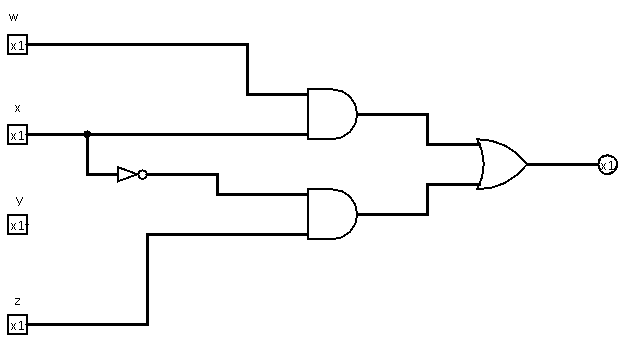
\includegraphics[scale=0.5]{Jminsop-01}
\caption{Circuit diagram of the minimal SOP solution of $J$.}
\label{fig:Jminsop-01}
\end{figure}

TODO: Similar to $J$, how is this done for $K$?
(Figure \ref{fig:Kminsop-01})

\begin{figure}[!htb]
\center
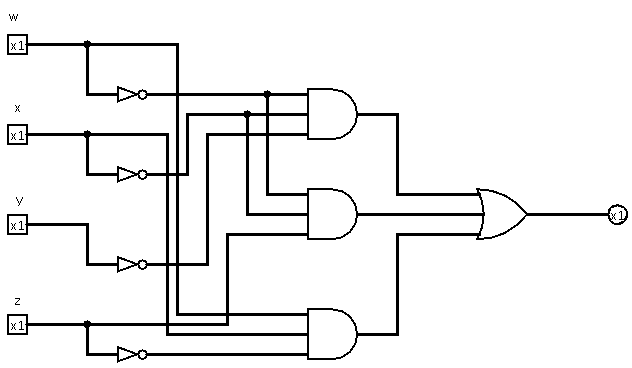
\includegraphics[scale=0.5]{Kminsop-01}
\caption{Circuit diagram of the minimal SOP solution of $K$.}
\label{fig:Kminsop-01}
\end{figure}

TODO: What about the version $K$ limited to 2 input gates?
(Figure \ref{fig:Kminsop-02})

\begin{figure}[!htb]
\center
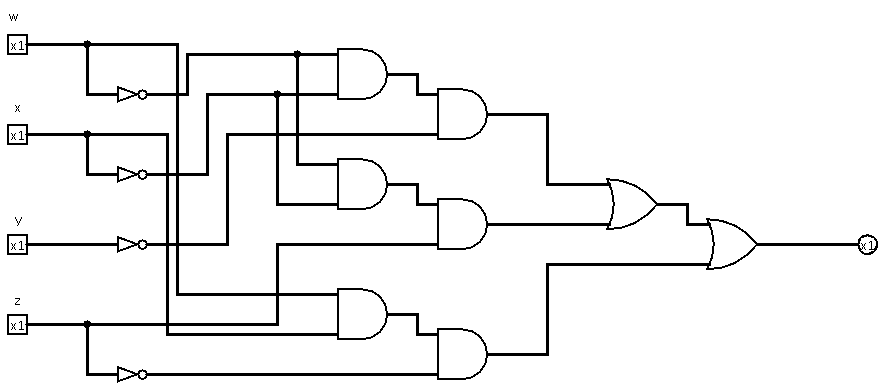
\includegraphics[scale=0.5]{Kminsop-02}
\caption{Circuit diagram of the minimal SOP solution of $K$ when limited to two input gates.}
\label{fig:Kminsop-02}
\end{figure}

\clearpage

TODO: What about for the jointly optimized solution of $J$ and $K$?
(Figure \ref{fig:JKjointkmap})
(Equation \ref{eq:JKjoint})

\begin{align}
	J &= w'x'z + wxz' + wz  \notag \\
	K &= w'x'z + wxz' + w'x'y'  \label{eq:JKjoint}
\end{align}

\begin{figure}[!htb]
\center
%\karnaughmap{4}{$J(w,x,y,z)$:}{wxyz}{0101000001011111}{}
%\karnaughmap{4}{$K(w,x,y,z)$:}{wxyz}{1101000000001010}{}
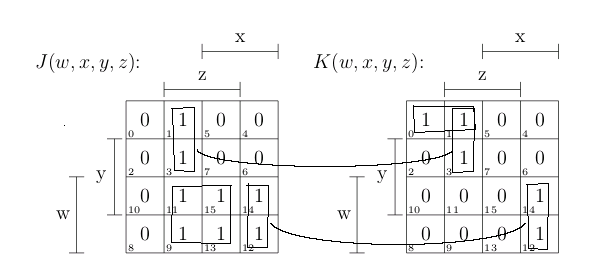
\includegraphics[scale=0.60]{JKkmap-01}
\caption{Jointly optimized Karnaugh maps for $J$ and $K$.}
\label{fig:JKjointkmap}
\end{figure}

TODO: How many gates, how many inputs for the joint solution?
(Figure \ref{fig:JKjointcircuit}).

\begin{figure}[!htb]
\center
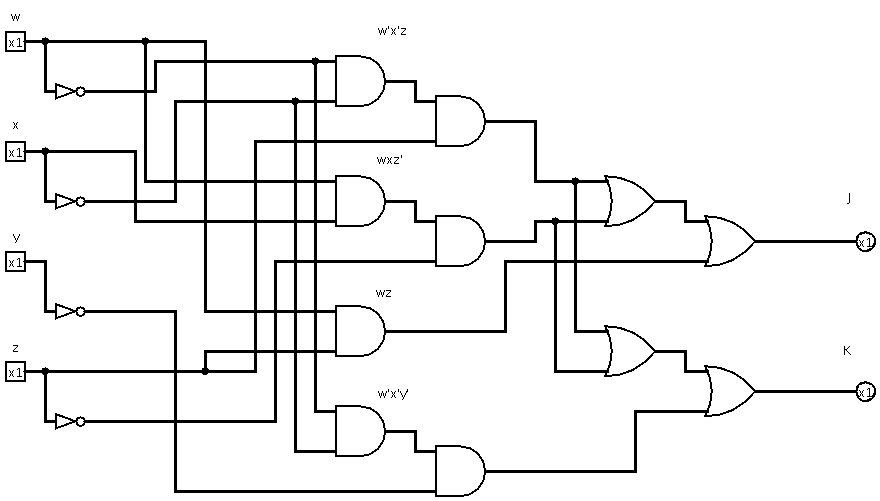
\includegraphics[scale=0.5]{JKjoint-01}
\caption{Circuit diagram of the jointly optimized solution of $J$ and $K$ when limited to two input gates.}
\label{fig:JKjointcircuit}
\end{figure}

TODO: describe the hardware implementation.
(Figure \ref{fig:JKjointcircuit}

\clearpage

\section{Observations}

TODO: How do the counts of various implementations compare?
Does the resulting function match the truth table?

\begin{table}[!htb]
\center
\begin{tabular}{cc}

\begin{tabular}{lll}
\multicolumn{3}{c}{\bf{$J$ by itself}} \\
gate type & \# gates & \# inputs\\
\hline
AND & 2 & 4\\
OR  & 1 & 2\\
NOT & 1 & 1 \\
\hline
\bf{TOTAL} & 4 & 7
\end{tabular}

&

\begin{tabular}{lll}
\multicolumn{3}{c}{\bf{$J$ and $K$ independently}} \\
gate type & \# gates & \# inputs\\
\hline
AND & 8 & 16 \\
OR  & 3 & 6  \\
NOT & 5 & 5  \\
\hline
\bf{TOTAL} & 16 & 27
\end{tabular}
\\
\\

\begin{tabular}{lll}
\multicolumn{3}{c}{\bf{$K$ by itself, 2 input gates}} \\
gate type & \# gates & \# inputs\\
\hline
AND & 6 & 12 \\
OR  & 2 & 4  \\
NOT & 4 & 4  \\
\hline
\bf{TOTAL} & 12 & 20
\end{tabular}

&

\begin{tabular}{lll}
\multicolumn{3}{c}{\bf{$J$ and $K$ jointly}} \\
gate type & \# gates & \# inputs\\
\hline
AND & 7 & 14 \\
OR  & 4 & 8  \\
NOT & 4 & 4  \\
\hline
\bf{TOTAL} & 15 & 26
\end{tabular}

\end{tabular} % outer formatting table

\caption{Metrics of gate and input counts for various configurations
of $J$ and $K$.}
\label{tbl:counts}
\end{table}


\section{Conclusion}

TODO: Was this lab a success in achieving the objective?

% flush all the figures
%\clearpage

% Uncomment these if you have references,
%\pagebreak
%\renewcommand*{\refname}{\vspace{-8mm}}
%\section{References}
%%\bibliographystyle{plain}
%%\bibliographystyle{mslapa}
%\bibliographystyle{ieeetr}
%\bibliography{../references}

% Appendix (if needed)

\end{document}

% vim:foldmethod=marker
